\documentclass[main.tex]{subfiles}

\begin{document}


\section{Практика 14.09.2022 (Базыров И.Ш.)}

\subsection{Закон Дарси}

В XIX веке наука во Франции была передовой.
В 1856 году в работе Дарси "<Les fontaines publiques de la ville de Dijon. Paris 1856"> (Общественные фонтаны города Дижон. Париж 1856) опубликованы результаты опытов по фильтрации воды в песке.
Опубликован закон, связывающий скорость фильтрации жидкости в пористой среде с градиентом давления.
Является основополагающим законом, который используется в гидродинамике.

До Дарси считалось, что поток в трубе не зависит от диаметра трубы и шероховатости её стенок. Это большое заблуждение, которое опровергли Дарси и Вейсбах.
На самом деле, потери напора в трубе связаны со скоростью в квадрате и есть коэффициент местного сопротивления (коэффициент потерь), который показывает изменение потерей напора на всём протяжении трубы (эти потери прямо пропорциональны длине трубы и обратно пропорциональны диаметру трубы).

Закон Дарси применим для фильтрации жидкостей, подчиняющихся закону вязкого трения Ньютона (закону Навье-Стокса).
Для фильтрации неньютоновских жидкостей (например, некоторых нефтей) связь между градиентом давления и скоростью фильтрации может быть нелинейной или вообще неалгебраической (например, дифференциальной).

Для ньютоновских жидкостей область применения закона Дарси ограничивается малыми скоростями фильтрации (числа Рейнольдса, рассчитанные по характерному размеру пор, меньше или порядка единицы).
При больших скоростях зависимость между градиентом давления и скоростью фильтрации нелинейна (хорошее совпадение с экспериментальными данными даёт квадратичная зависимость -- закон фильтрации Форхгеймера).

Основные допущения закона Дарси:

1) постоянный дебит;

2) ламинарное течение;

3) гомогенная среда фильтрации;

4) поровое пространство насыщенно одной фазой;

5) отсутствие химического взаимодействия между породой и флюидом.

\subsubsection{Линейное течение}


\subsubsection{Радиальное течение. Формула Дюпюи}

Дюпюи решил дифференциальное уравнение для случая границы в виде цилиндрической области (для радиального режима течения).

\beq
\frac{Q}{A}=\frac{k}{\mu}\frac{dP}{dx}\Rightarrow\frac{Q}{2\pi h}\int\limits_{r_w}^{r_e}{\frac{dr}{r}}=\frac{k}{\mu}\int\limits_{P_w}^{P_e}{dp}\Rightarrow Q=\frac{2\pi kh}{\mu}\frac{P_e-P_w}{\ln{\left(\dfrac{r_e}{r_w}\right)}}
\eeq

\subsection{Скин-фактор}

Для корректной оценки притока (калибровки модели к реальным данным) необходимо также учесть дополнительный перепад давления в призабойной зоне, то есть скин-фактор:
\beq
S=\dfrac{\Delta P_s}{\dfrac{Q\mu}{2\pi kh}}
\eeq

\beq
P_{wf}=P_e-\frac{Q\mu}{2\pi kh}\left(\ln{\left(\frac{r_e}{r_w}\right)}+S\right)
\eeq
В дальнейшем скин-фактор используется инженерами для учёта не только перепада давления в призабойной зоне.


\subsection{Формула Дюпюи с учётом скин-эффекта}

\beq
Q=\frac{kh}{18.41\cdot\mu}\frac{P_e-P_w}{\ln{\left(\dfrac{r_e}{r_w}\right)}+S}
\eeq

\subsection{Определение дебита по формуле Дюпюи, анализ чувствительности}

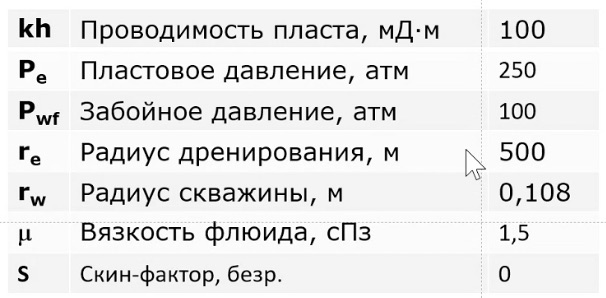
\includegraphics[width=0.4\textwidth]{input_for_Dupuy}

Здесь $P_e$ -- пластовое давление на границе области дренирования.

\beq
Q=\frac{kh}{18.41\cdot\mu}\frac{P_e-P_w}{\ln{\left(\dfrac{r_e}{r_w}\right)}+S}=
\frac{100\text{ мД}\cdot\text{м}}{18.41\cdot 1.5\text{ сПз}}\frac{250\text{ атм}-100\text{ атм}}{\ln{\left(\dfrac{500\text{ м}}{0.108\text{ м}}\right)}+0}\approx64\frac{\text{м}^3}{\text{сут}}
\eeq

\subsection{Задача 1}

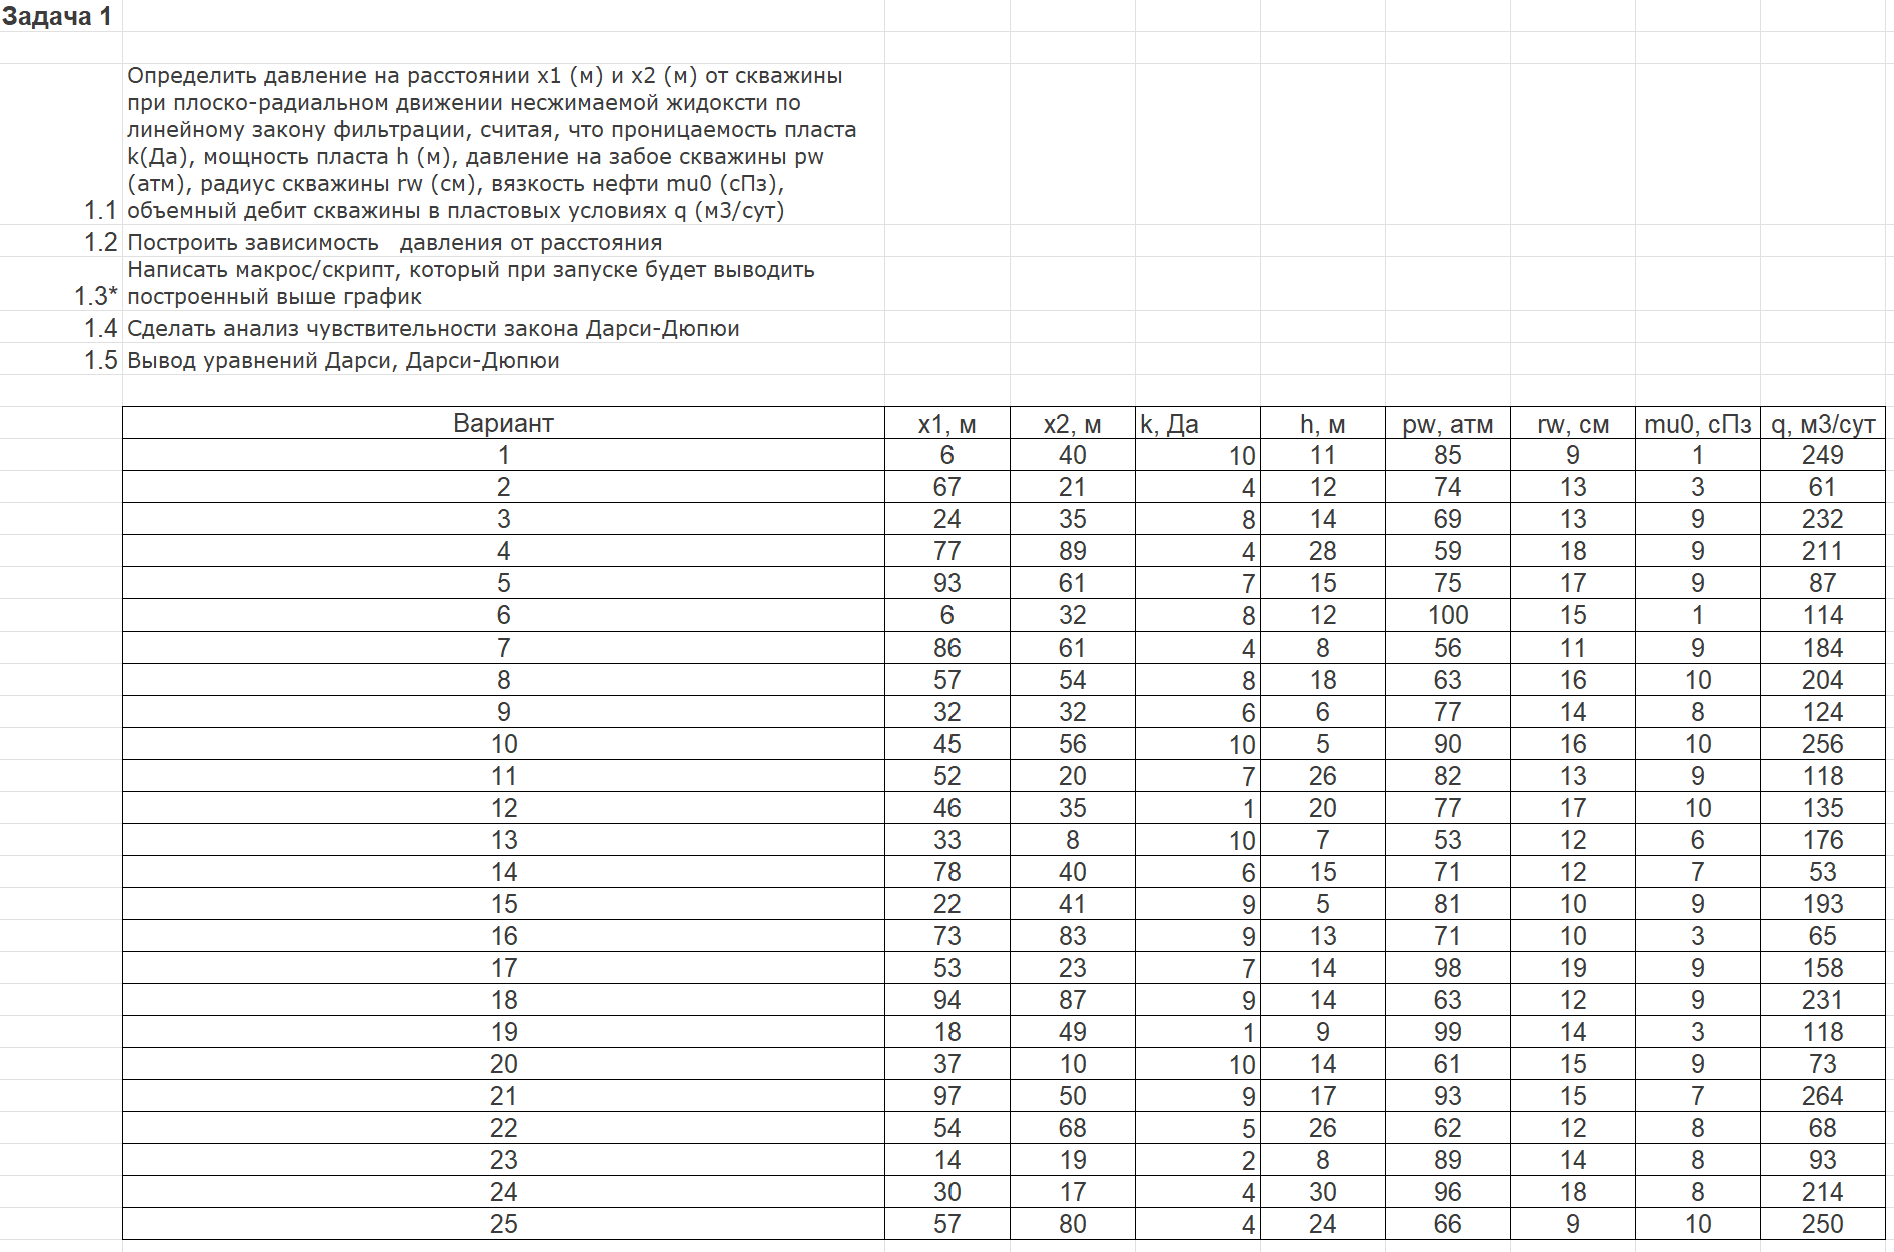
\includegraphics[width=\textwidth]{task1}

Вариант 16.

Давление на расстоянии $x_1$:
\begin{multline}
P_{x_1}=P_w+\frac{18.41\cdot Q\mu}{kh}\left(\ln{\left(\frac{x_1}{r_w}\right)+S}\right)
=\\=71\text{ атм}+\frac{18.41\cdot 65\dfrac{\text{м}^3}{\text{сут}}\cdot3\text{ сПз}}{9000\text{ мД}\cdot 13\text{ м}}\left(\ln{\left(\frac{73\text{ м}}{0,1\text{ м}}\right)}+0\right)\approx 71.2\text{ атм}
\end{multline}

Давление на расстоянии $x_2$:
\begin{multline}
P_{x_1}=P_w+\frac{18.41\cdot Q\mu}{kh}\left(\ln{\left(\frac{x_2}{r_w}\right)+S}\right)
=\\=71\text{ атм}+\frac{18.41\cdot 65\dfrac{\text{м}^3}{\text{сут}}\cdot3\text{ сПз}}{9000\text{ мД}\cdot 13\text{ м}}\left(\ln{\left(\frac{83\text{ м}}{0,1\text{ м}}\right)}+0\right)\approx 71.2\text{ атм}
\end{multline}

График зависимости давления от расстояния построен по ссылке: \href{https://colab.research.google.com/github/mualal/notebooks-source/blob/master/6_pressure.ipynb}{Open in Colab}.

\subsection{Что такое гидродинамическое моделирование?}

См. вводную лекцию.

\subsection{Уравнение пьезопроводности (без упругости пласта)}

См. вводную лекцию.

\subsection{Решение линейного стока/источника в однородном бесконечном коллекторе}

Для вывода решения используются безразмерные переменные. Например, безразмерные радиус, время и давление:

\beq
r_D=\frac{r}{r_w};\,\,\,\,\,\,\,\,t_D=\frac{kt}{\varphi c_t r_w^2};\,\,\,\,\,\,\,\,P_D=\frac{2\pi kh}{qB\mu}\left(p_i-p\right)
\eeq

Преимущества использования безразмерных переменных:

1) вид уравнений упрощается;

2) полученное один раз решение можно использовать для самых разных конфигураций;

3) безразмерные переменные -- основа для метода палеточной интерпретации.

Решение в безразмерных переменных, записанное через интегральную показательную функцию:
\beq
P_D(r_D,t_D)=-Ei\left(-\frac{r_D^2}{4t_D}\right),
\eeq
где
\beq
-Ei(-x)=\int\limits_{x}^{\infty}\frac{e^{-u}}{u}du.
\eeq

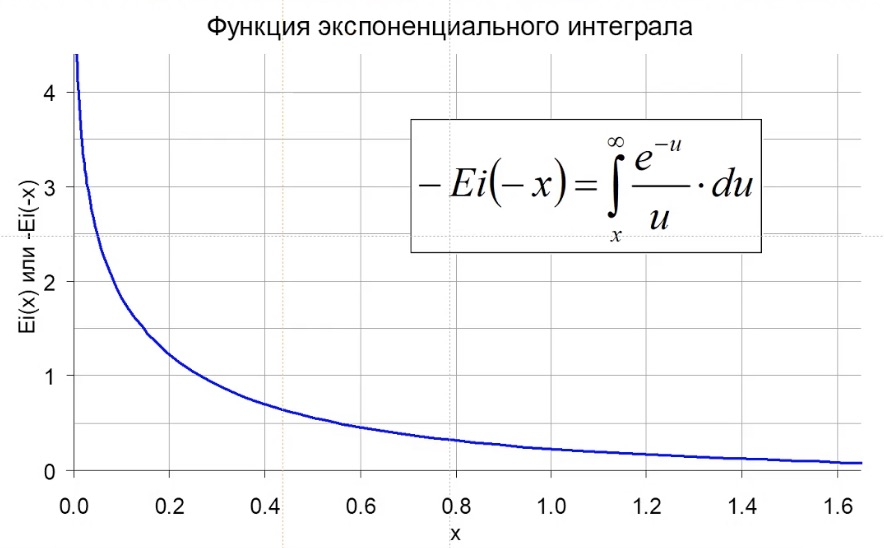
\includegraphics[width=0.5\textwidth]{exp_integral}

Логарифмическая аппроксимация решения при условии $\dfrac{r_D^2}{4t_D}\leqslant0.01$:
\beq
P_D(r_D,t_D)\approx -\frac{1}{2}\left[\ln\frac{\gamma r_D^2}{4t_D}\right]=\frac{1}{2}\left[\ln\frac{t_D}{r_D^2}+0.80907\right].
\eeq

Решение линейного стока:
\beq
P(r,t)=p_i-\frac{qB\mu}{2\pi kh}\left[-\frac{1}{2}Ei\left(-\frac{\varphi\mu c_t r^2}{4kt}\right)\right].
\eeq

Логарифмическая аппроксимация решения при условии $\dfrac{kt}{\varphi \mu c_t r^2}\geqslant25$:
\beq
P(r,t)\approx p_i-\frac{1}{2}\frac{qB\mu}{2\pi kh}\left[\ln\frac{kt}{\varphi\mu c_t r^2}+0.80907\right].
\eeq

\subsection{Что такое модель, или зачем нужно решать уравнение пьезопроводности?}

\beq
P(r,t)\approx p_i-\frac{1}{2}\frac{qB\mu}{2\pi kh}\left[\ln\frac{kt}{\varphi\mu c_t r^2}+0.80907\right].
\eeq

Уравнение пьезопроводности -- основа аналитических моделей пласта, использующихся в различных симуляторах (например, в Saphir).

\subsection{Задача 2}

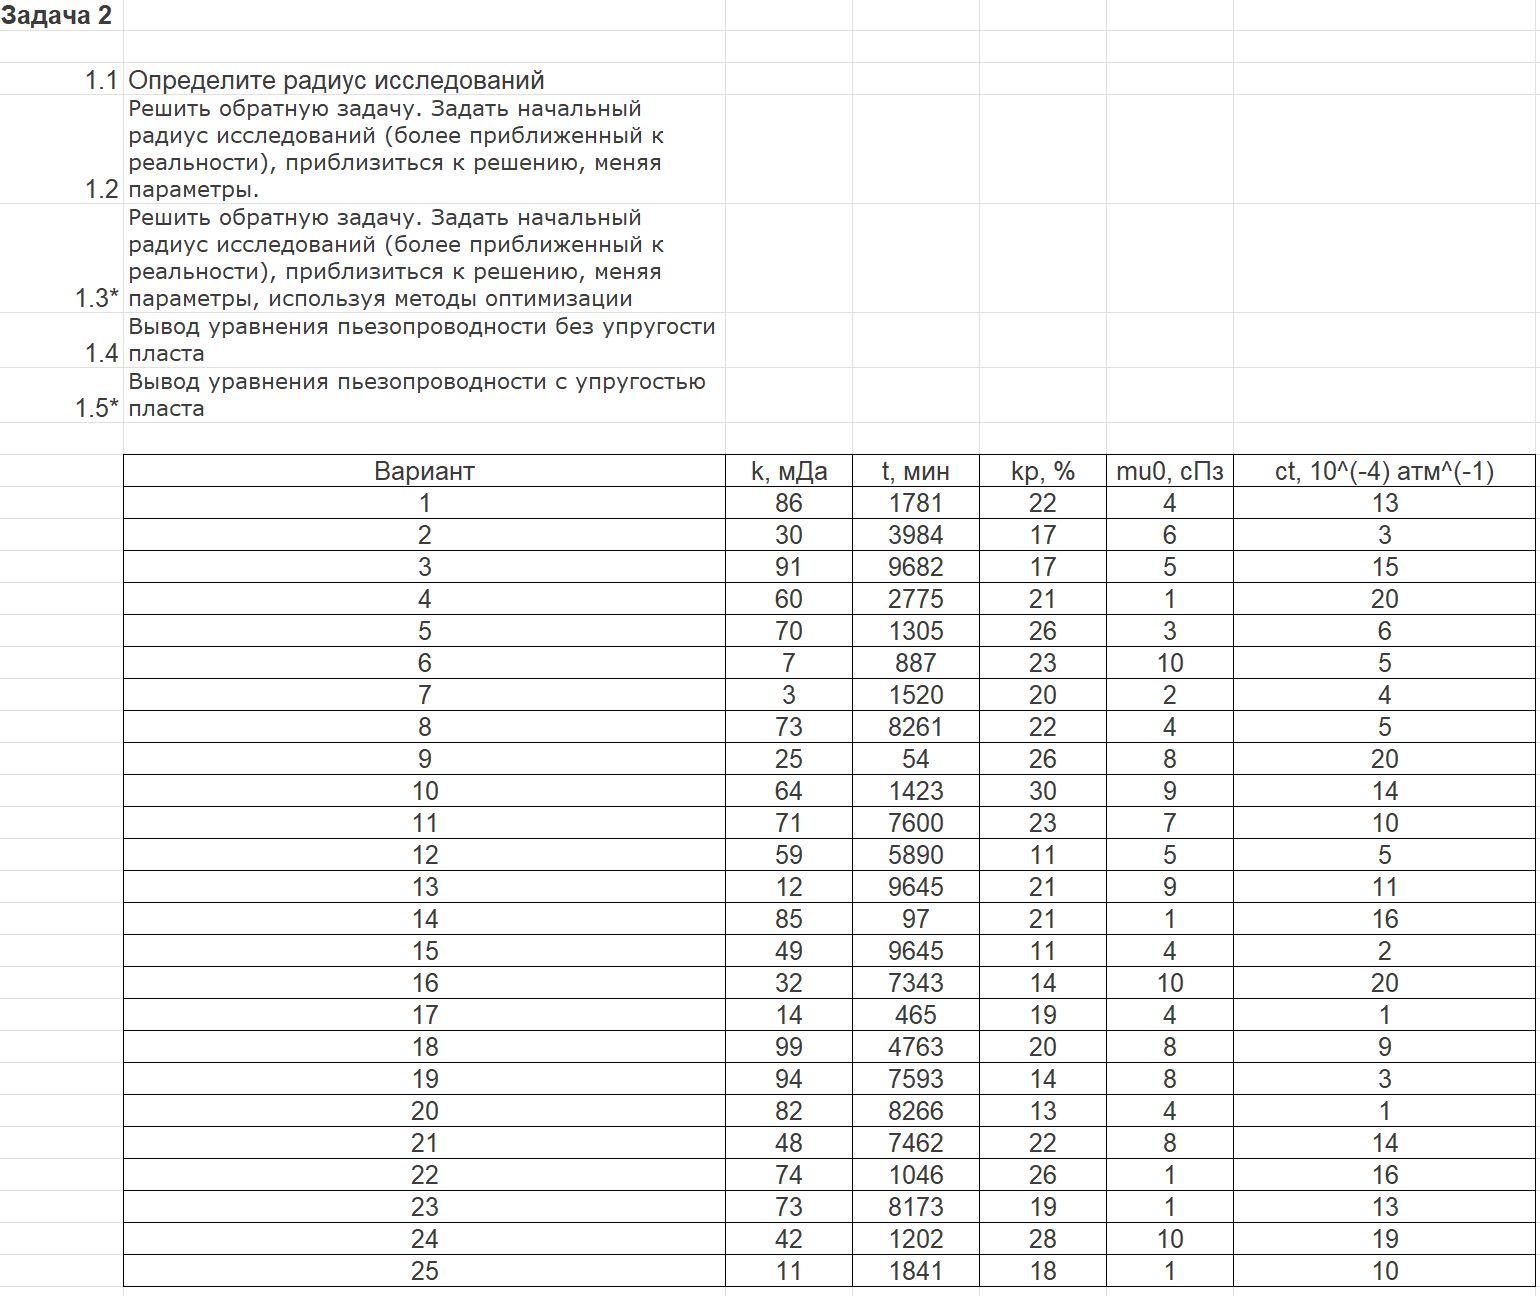
\includegraphics[width=\textwidth]{task2}

Вариант 16.

\beq
r_{inv}=0.037\sqrt{\frac{kt}{\varphi \mu c_t}}=0.037\sqrt{\frac{0.032\text{ Да}\cdot 7343\cdot 60\text{ с}}{0,14\cdot 0.10\text{ Пз}\cdot 20\cdot 10^{-4}\dfrac{\text{1}}{\text{атм}}}}\approx 830\text{ см}=8.3\text{ м}
\eeq

График зависимости радиуса исследования от произведения проницаемости и времени построен по ссылке: \href{https://colab.research.google.com/github/mualal/notebooks-source/blob/master/7_exploration_radius.ipynb}{Open in Colab}.

%Проведём проверку размерностей, выражая каждую через основные единицы системы НПГ:

%\beq
%\sqrt{\frac{}{}}
%\eeq


\end{document}
